\documentclass{beamer}

\usepackage[utf8]{inputenc}
\usepackage[T1]{fontenc}
\usepackage{amsmath}
\usepackage{bm}

\usepackage{tabularx}
\usepackage{graphicx}
\usepackage{epstopdf}
\usepackage{multirow}

\graphicspath{{../../images/}}

\usetheme{Madrid}
\usebeamercolor{sidebartab}
\usefonttheme{professionalfonts}


\title[M.Sc. Thesis 2015]{Spatial Summarization of Image Collections}
\author{Diego A. Ballesteros Villamizar}
\institute[ETHZ]{ETH Zürich}
\date{February 22nd, 2016}

\DeclareMathOperator*{\argmin}{argmin}
\DeclareMathOperator*{\argmax}{argmax}

\AtBeginSection[]
{
  \begin{frame}<beamer>
    \frametitle{Outline}
    \tableofcontents[currentsection]
  \end{frame}
}

\begin{document}

\begin{frame}
  \titlepage
\end{frame}

\section{Analysis of the evaluation}

\begin{frame}{Strict evaluation for Markov model}
  \begin{itemize}
    \item The test set is generated ensuring that the last element is the element before the one that was removed from the set.
    \item Previously the order was not preserved and the ranking from the model was obtained summing the transition probabilities starting from each element in the partial set.
    \item This is the evaluation for the Markov model from now on.
      \begin{table}
        \begin{tabular}{@{}lll@{}}
          \hline
          \textit{Model (N = 10)} & \textit{Accuracy} & \textit{MMR} \\
          \hline
          Markov & $27.93 \pm 3.02$ & $51.03 \pm 1.86$ \\
          Markov (prev.) & $32.07 \pm 2.69$ & $52.40 \pm 1.76$ \\
          Markov with heuristic & $39.74 \pm 3.62$ & $60.64 \pm 1.98$ \\
          Markov with heuristic (prev.) & $36.50 \pm 3.10$ & $57.91 \pm 1.89$ \\
          \hline
        \end{tabular}
      \end{table}
  \end{itemize}
\end{frame}

\begin{frame}{Evaluation over different partial set sizes}
  \begin{figure}
    \centering
    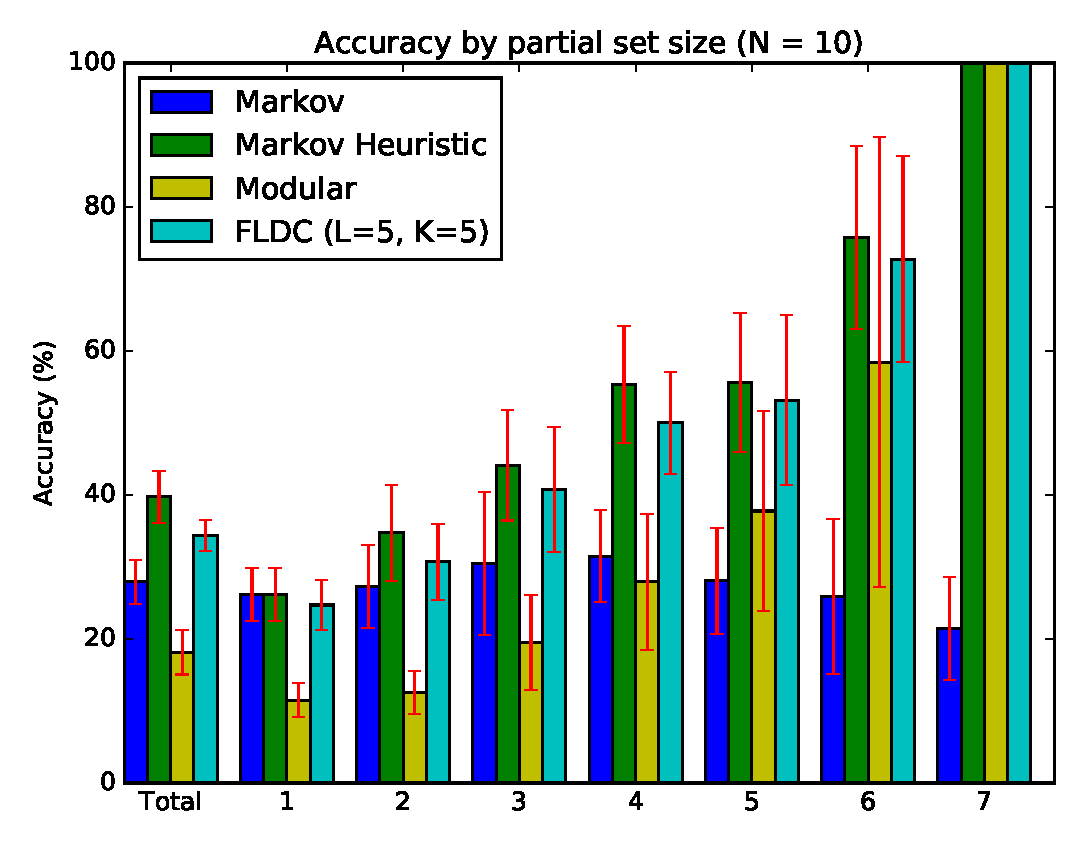
\includegraphics[width=0.8\textwidth]{set_size_score_10}
  \end{figure}
\end{frame}

\begin{frame}{Evaluation over different partial set sizes}
  \begin{figure}
    \centering
    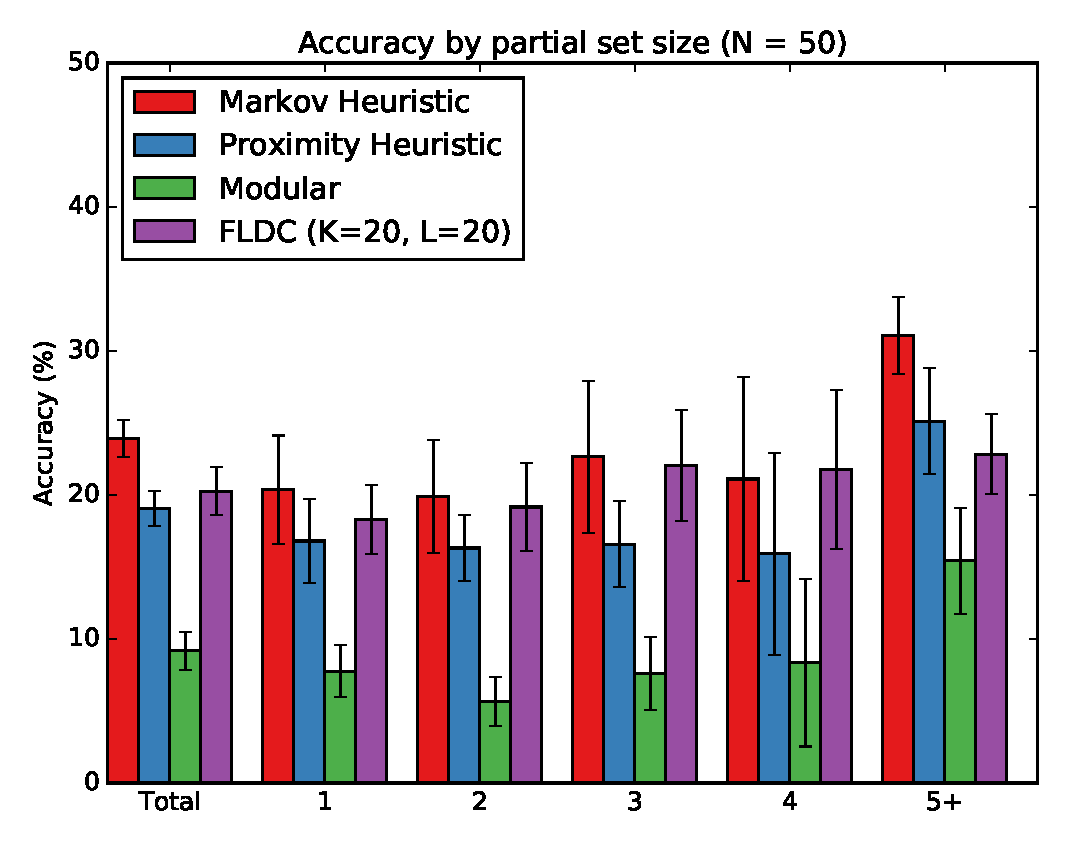
\includegraphics[width=0.8\textwidth]{set_size_score_50}
  \end{figure}
\end{frame}

\section{Changing the learning}

\begin{frame}{Learning from elements with at least 2 elements}
  \begin{itemize}
    \item From now on the the number of items (i.e. mean-shift clusters) is 50.
    \item Removing all singletons from the data leaves 2832 paths/sets. Including singletons the count is 12614.
    \item For each fold the train set size is: 2548 and the test set size is: 284.
  \end{itemize}
\end{frame}

\begin{frame}{Results comparison}
  \begin{columns}
    \begin{column}{0.5\textwidth}
      \begin{figure}
        \centering
        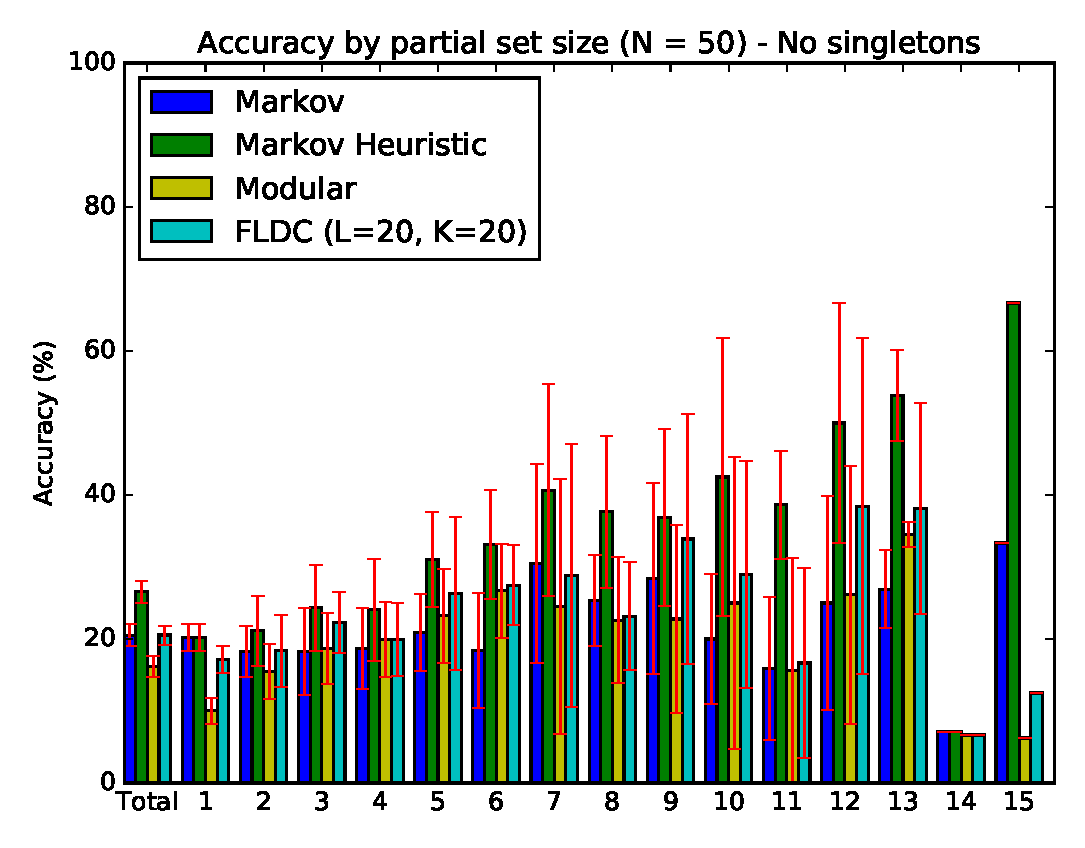
\includegraphics[width=\columnwidth]{set_size_score_50_no_singles}
      \end{figure}
    \end{column}
    \begin{column}{0.5\textwidth}
      \begin{figure}
        \centering
        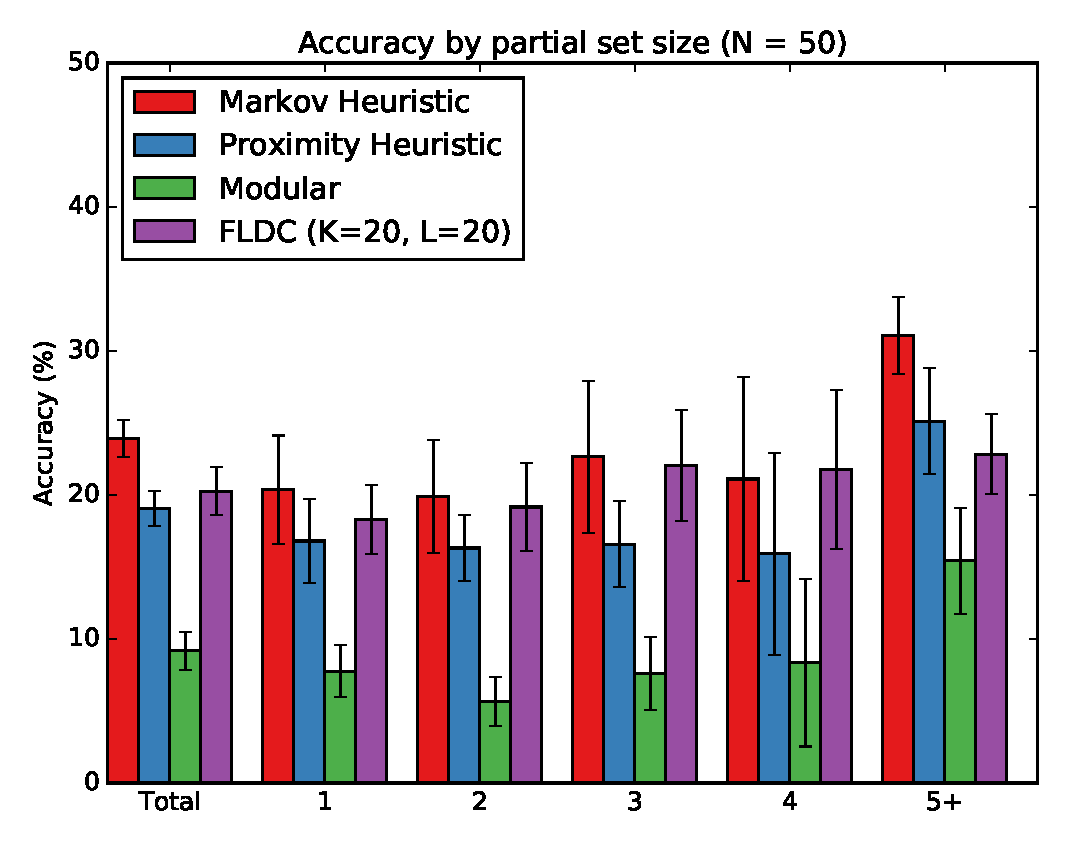
\includegraphics[width=\columnwidth]{set_size_score_50}
      \end{figure}
    \end{column}
  \end{columns}
\end{frame}

%\begin{frame}{References}
%  \bibliographystyle{acm}
%  \bibliography{../references}
%\end{frame}

\end{document}
